\documentclass[11pt]{beamer}
\usepackage{enumitem,xcolor}
\usepackage{ulem}
\usepackage{natbib}
\usepackage[utf8]{inputenc}

\beamertemplatenavigationsymbolsempty
\usecolortheme{beaver}

% Citation styles
\bibliographystyle{apalike}
\setcitestyle{authoryear, open={(}, close={)}}

\newlist{coloritemize}{itemize}{1}
\setlist[coloritemize]{label=\textcolor{itemizecolor}{-}}
\colorlet{itemizecolor}{.}

% $\checkmark$

\title{Proto-Word Reconstruction with RNNs}
\subtitle{Project Sketch}
\date{\today}
\author{Julius Steuer \and Morgan Wixted}

%--------------------------------------------------------------------------------------------------
%--- Title
%--------------------------------------------------------------------------------------------------
\begin{document}
\begin{frame}[plain]
    \small
    Software Project NLP with NNs
    \normalsize
    \titlepage
\end{frame}

%--------------------------------------------------------------------------------------------------
%--- Goal
%--------------------------------------------------------------------------------------------------
\begin{frame}
    \frametitle{Goal of the Project}
    \begin{itemize}
        \item[--] Provide a tool to automatically reconstruct proto-words for a given sample of cognate sets
        \item[--] Allow custom feature encoding \& transcription
        \item[--] Initial hypothesis if not much is known about the family
        \item[--] Allow for integration of linguistic knowledge
        \begin{itemize}
            \item[$\circ$] Alignment between cognate loci in different languages
            \item[$\circ$] Exclude word parts assumed to be innovations (e. g. spanish \textit{nos-otros} from latin \textit{no:s}) 
        \end{itemize}
        \item[--] Examine the influence of input representations on model performance (alignments, transcriptions) 
    \end{itemize}
\end{frame}
%--------------------------------------------------------------------------------------------------
%--- Meloni paper
%--------------------------------------------------------------------------------------------------
\begin{frame}
    \frametitle{Baseline}
    Start from \cite{meloni_ab_2019}: 
    \begin{itemize}
        \item[--] Romance dataset (not publicly availabe)
        \item[--] Character-based encoder-decoder architecture with Bahdanau attention
        \item[--] Characters encoded as 100-bit vectors (localist representation)
        \item[--] Output one character of the reconstructed word per timestep 
        \item[--] Evaluate impact of individual languages on reconstruction:
        \newline
        \begin{figure}[t]
            \centering
            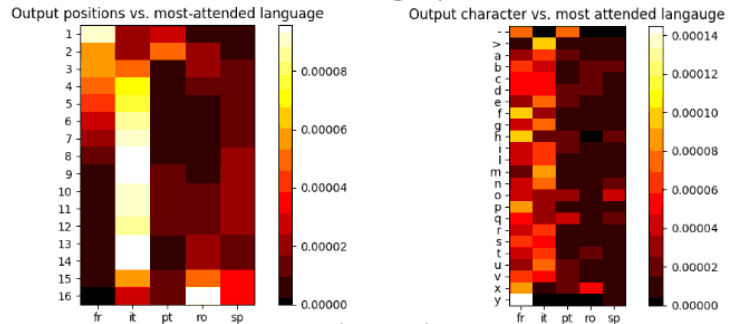
\includegraphics[width=0.7\textwidth]{graphics/meloni_figure_4.png} 
        \end{figure}
    \end{itemize}
\end{frame}

%--------------------------------------------------------------------------------------------------
%--- Model
%--------------------------------------------------------------------------------------------------
\begin{frame}{Model}
    Idea:
    \begin{itemize}
        \item[--] Use distributed feature encodings to represent characters, not embeddings
        %\item[--] Use the stem of the Latin word as the proto-form, since nominative inflection is seldom preserved in modern Romance 
        \item[--] Start with ASJP (easily available) transcriptions (\cite{brown_automated_2008}), then use IPA
        \item[--] Pairwise alignments of sequence chunks (following \cite{ciobanu_ab_2018}) \\
        \begin{center}
        \begin{tabular}{lcccccccccc}
            \hline
            \multicolumn{11}{c}{Latin acc. sing \textit{corticem} 'bark' $\rightarrow$ ASJP \{kortike\}} \\
            \hline
            & 1 & 2 & 3 & 4 & 5 & 6 & 7 & 8 & 9 & 10 \\
            latin & - & k & o & - & r & t & i & k & - & e \\
            italian & - & k & o & - & r & t & e & t & C & a \\
            spanish & - & k & o & - & r & t & e & 8 & - & a \\
            french & e & k & o & - & r & - & - & - & - & - \\
            romanian & s & k & o & a & r & - & - & c & - & 3  
        \end{tabular}
        \end{center}
    \end{itemize}
\end{frame}

\begin{frame}
    \frametitle{Model, feature encoding}
    \begin{figure}
        \centering
        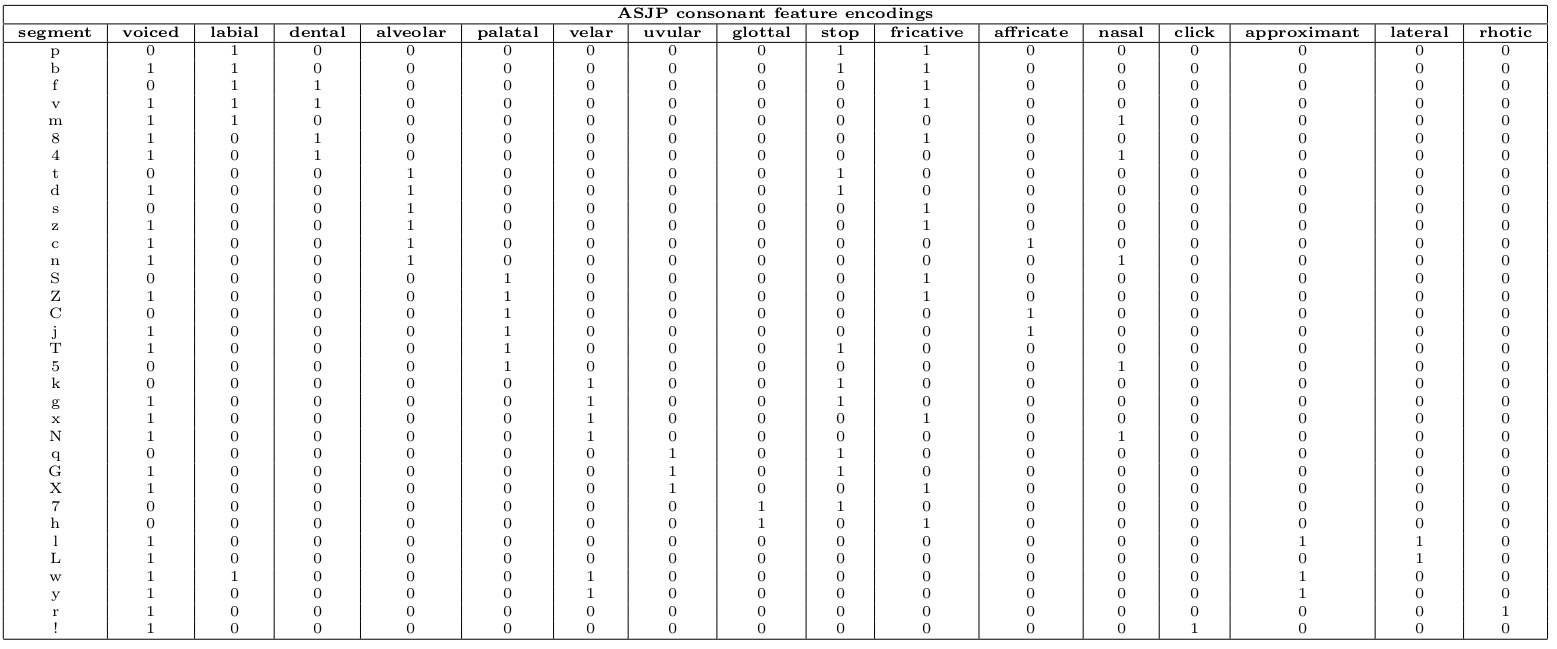
\includegraphics[scale=.21]{graphics/asjp_cons.png}
    \end{figure} 
    \begin{figure}[htp]
            \centering
            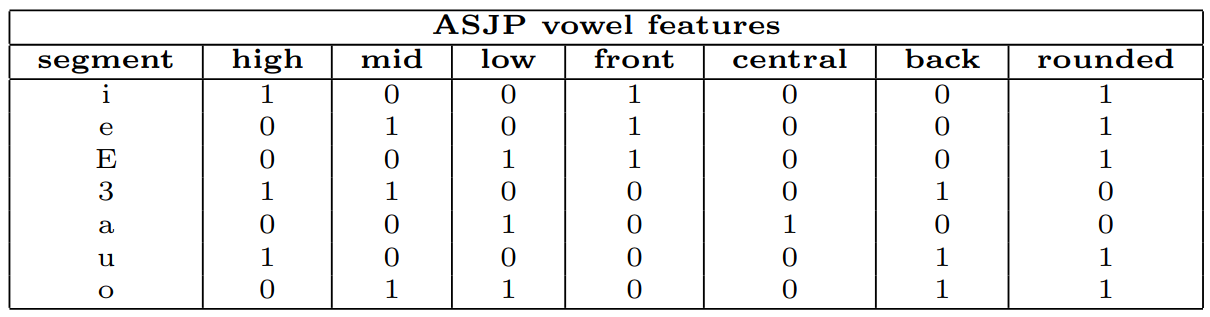
\includegraphics[width=0.6\textwidth ]{graphics/asjp_vowels.png}
    \end{figure}
 \end{frame}


\begin{frame}
    \frametitle{Model, continued}
    Input:
    \begin{itemize}
        \item[--] One column represents the input at a single timestep, latin character at that alignment position is the expected output:
        \newline
        \begin{center}
        \begin{tabular}{c|c|c}
            \textbf{T} & \textbf{I} & \textbf{O} \\
            \hline
            $t_{1}$ & (- ,- ,e, s) & - \\
            $t_{2}$ & (k, k, k, k) & k \\
            $\cdots$ & $\cdots$ \\
            $t_{10}$ & (a, a, -, 3) & e
        \end{tabular} 
        \end{center}
        %\begin{align*}
        %    I_{T=t_{1}} &= (-,-,e,s) \\
        %    I_{T=t_{2}} &= (k,k,k,k) \\
        %    \cdots \\
        %    I_{T=t_{10}} &= (a,a,-,3)
        %\end{align*} 
        \item[--] Attention: \cite{meloni_ab_2019} attend on different languages in the cognate set. \\
        $\rightarrow$ Either (as in the paper) perform a pass through the model to reconstruct a single character (each $I_{T=t_{i}}$ a sequence of inputs), or 
        \item[--] Use the matrix/vector $I_{T=t_{i}}$ at a single time step, and perform only one pass
    \end{itemize}
\end{frame}

\begin{frame}
    \frametitle{Model, limitations}
    But: The direct precursor of italian \textit{corteccia}, spanish \textit{corteza} etc. is the latin adjective \textit{corticeus, -a, -um}
    \begin{itemize}
        \item[--] We expect the model to reconstruct an a-stem noun instead of a consononat stem \text{cortex, cortices}
        \item[--] Spurious sounds (french \textit{e-}, romanian \textit{s-}) should be dropped (?)
        \item[--] Ambiguous sounds may not indicate a clear rule (latin \textit{-k-} vs. rom. \textit{-c-} vs. spanish \textit{-8-})  
    \end{itemize}
\end{frame}

%--------------------------------------------------------------------------------------------------
%--- Milestones
%--------------------------------------------------------------------------------------------------
\begin{frame}
    \frametitle{Milestones}
    Minimal:
    \begin{itemize}
        \item[--] Reconstruction with ASJP encodings, small Swadesh list as data 
        \item[--] \sout{Then switch to IPA encodings}  Using the epitran \footnote{https://github.com/dmort27/epitran} Python package to get IPA transcriptions
        \item[--] Try different language family (initial guess on unseen data)
        \item[--] Examinate the influence of differrent (or absent) alignments on model performance  
    \end{itemize}    
    Great to have:
    \begin{itemize}
        \item[--] \sout{Use larger dataset (ask Ciobanu for hers)} Use Ciobanu's dataset from 2014
        \item[--] Ensure compatibility with the LingPy \footnote{http://lingpy.org/} WordList 
        \footnote{http://lingpy.org/reference/lingpy.basic.html\#lingpy.basic.wordlist.Wordlist} class
        \item[--] Use LingPy to work with pre-aligned data (Austronesian)
    \end{itemize}
\end{frame}

%--------------------------------------------------------------------------------------------------
%--- Refs 
%--------------------------------------------------------------------------------------------------
\begin{frame}
    \frametitle{References}
    \bibliography{../bib/NLPwithNN.bib}
\end{frame}

\end{document}
